\documentclass{standalone}
\usepackage{amsmath}
\usepackage{pgfplots}
\pgfplotsset{compat=1.7}

\begin{document}
	
	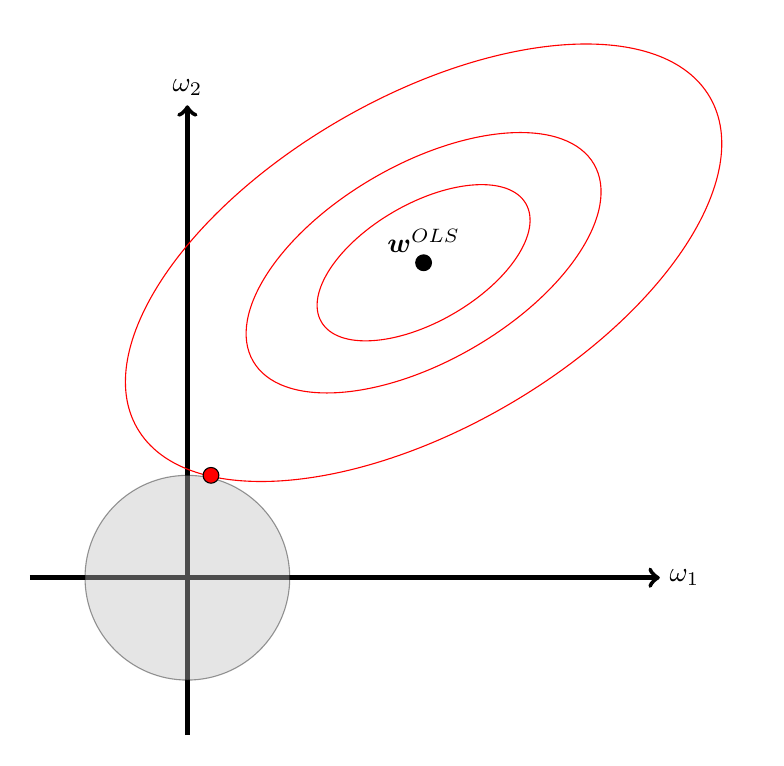
\begin{tikzpicture}
	\draw [ultra thick, ->] (-2,0)--(6,0);
	\node [right] at(6,0) {$\omega_1$};
	\draw [ultra thick, ->] (0,-2)--(0,6);
	\node [above] at(0,6) {$\omega_2$};
	\draw [fill=black] (3,4) circle [radius=0.1cm];
	\node[above] at(3,4) {$\boldsymbol{w}^{OLS}$};
	\draw[fill=lightgray, opacity=0.4] (0,0) circle [radius=1.3cm];
	\draw[rotate around={-60:(3,4)},red] (3,4) ellipse (0.75cm and 1.5cm);
	\draw[rotate around={-60:(3,4)},red] (3,4) ellipse (1.25cm and 2.5cm);
	\draw[rotate around={-60:(3,4)},red] (3,4) ellipse (2.1cm and 4.2cm);
	\draw [fill=red] (0.3,1.3) circle [radius=0.1cm];
	\end{tikzpicture}

\end{document}